\section{FrameNet}

\subsection{Semantische Frames}

FrameNet ist eine lexikalische Ressource, die in der Universität Berkeley entwickelt wurde und  auf der sprachwissenschaftlichen Theorie der Frame-Semantik nach Charles J. Fillmore basiert (\cite[vgl.][1]{NLTKPROJEKT}).
\par
Um ein Wort oder eine abstrakte Idee begreifen zu können, aktiviert das menschliche Gehirn einen Deutungsrahmen (engl. \textit{frame}). Der Inhalt dieses Frames leitet sich aus dem bestehenden Wissens- und Erfahrungsschatz der jeweiligen Person ab (\cite[vgl.][28]{WEHLING}). Bei dem Wort \textit{tanzen} assoziiert der Leser in der Regel direkt in Verbindung stehende Ideen wie Musik, Choreografie und sich bewegende Menschen. Ein Frame beinhaltet folglich ein ganzes Bündel an Informationen.
\par
Auslöser für die Aktivierung eines Frames sind \textit{Lexical Units}. Hierbei handelt es sich um Wort-Sinnpaare, also um ein Wort und ganz konkretes Verständnis dieses Wortes (\cite[vgl.][1]{NLTKPROJEKT}). Beispielsweise kann das Wort \textit{treffen}, im Sinne von \textit{begegnen}, den Frame \textit{Begegnung} aktivieren, mit dem in der Regel zwei Personen, Händeschütteln oder Grußworte assoziiert werden. \textit{Treffen} im Sinne von \textit{ein Ziel treffen} erweckt ganz andere Erinnerungen und somit einen anderen Frame. Bei der aktivierenden Lexical Unit muss es sich jedoch nicht zwangsläufig um ein einzelnes Wort halten. Auch Ausdrücke mit mehreren Wörtern können eine Lexical Unit bilden.
\par
Als Valenz wird die Fähigkeit eines Wortes bezeichnet, andere Wörter an sich zu binden. Ein Valenzmuster ist somit eine syntaktische Schablone für den üblichen Gebrauch eines Wortes. Wird ein Wort in einem Satz ohne Berücksichtung der in der jeweiligen Sprache üblichen Valenzmuster eingebaut, klingt das Resultat falsch oder ungewohnt.
\par
Die mit einem Frame assoziierten Vokabeln werden als \textit{Frame Elemente} bezeichnet. Über sie steht der Frame in Verbindung mit anderen Frames. 

\subsection{Aufbau und Struktur}

Ähnlich wie WordNet, ist FrameNet ebenfalls als azyklischer Graph strukturiert. Die Knoten bilden jedoch nicht Synsets, sondern Frames under deren Frame Elemente. Die Beziehungen zwischen den Frames sind die Kanten. FrameNet ist weniger granular als WordNet in der Unterscheidung von Wortbedeutungen. Ähnlich wie in WordNet existieren auch in FrameNet verschiedene Beziehungstypen.
\par
Die Vererbungsrelation \textit{Inheritance} stellt eine IS-A-Relation dar. Jedes Frame Element im Eltern-Frame ist mit koresspondierenden Frame-Elementen im Kind-Frame verbunden. Ein \textit{Subframe} stellt ein Subevent zu einem komplexeren oder abstrakten Eltern-Frame dar. Der 
\textit{Using}-Beziehungstyp nutzt den Eltern-Frame als Hintergrund. Nicht alle Eltern-Frame-Elemente müssen jedoch mit Kinde-Frame-Elementen verbunden sein. Darüber hinaus gibt es noch weitere, seltener auftretende Beziehungstypen.


\subsection{Semantic Role Labeling}

Ein Hauptanwendungsgebiet für FrameNet ist das \ac{SRL}. Hierbei wird einem Satzglied, in der Linguistik auch als \textit{Argument} bezeichnet, eine abstrakte Rolle zugewiesen. Die semantische Satzaussage, das \textit{Prädikat}, ergibt sich dann aus der Summe der Argumente. Aus diesem flachen semantischen Repräsentationslevel können dann Informationen extrahiert werden.
\par
Ein Problem des \ac{SRL} ist die einheitliche Definition von Rollen. Abhängig vom Abstraktonsgrad können konkrete Rollendefinitionen (\textit{Deep Roles}) oder abstrakte Rollendefinitionen (\textit{Thematic Roles}) verwendet werden. Typische Beispiele für thematische Rollen sind beispielsweise (\cite[vgl.][379]{JURAFSKY}):
\begin{itemize}
\item AGENT: Verursache eines Ereignisses.
\item THEME: Direkt vom Ereignis beeinflusstes Satzglied
\item INSTRUMENT: In einem Ereignis verwendeter Gegenstand
\item GOAL: Ziel eines Objektes in einem Transferevent.
\end{itemize}

Die tatsächlich verwendeten Rollendefinitionen unterschieden sich von Implementierung zu Implementierung.

\begin{wrapfigure}{!ht}{8cm}
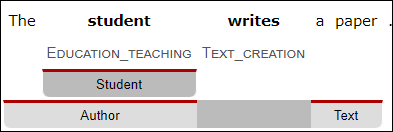
\includegraphics[width=7cm]{pictures/SEMAFOR1.png}
\caption{SRL: Aktiv}
\label{fig:SEMAFOR1}
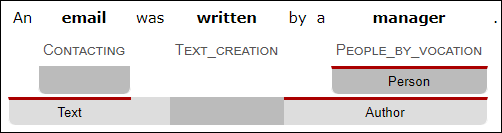
\includegraphics[width=7cm]{pictures/SEMAFOR2.png}
\caption{SRL: Passiv}
\label{fig:SEMAFOR2}
\end{wrapfigure}

Die semantischen Rollen stehen nicht zwangsläufig in Beziehung zu der syntaktischen Rolle der Satzglieder. Abbildung  \ref{fig:SEMAFOR1} zeigt den \textit{student} als Subjekt des Satzes. Abbildung \ref{fig:SEMAFOR2} zeigt das \textit{paper} als Subjekt des Satzes.
In beiden Fällen erfüllt der \textit{student} die Rolle des Authors und das \textit{paper} die Rolle des Textes. Die Abbildungen wurden mit dem Webeditor der Tools SEMAFOR (http://\-demo\-.ark\-.cs\-.cmu\-.edu) erzeugt.
\par
Eine solche Veränderung der Argumentreihenfolge wird als \textit{Diathesis Alternation} bezeichnet. Die Menge der möglichen Argumentfolgen die zu einem bestimmten Verb gehören werden als \textit{Thematic Grid} oder \textit{Case Frame} bezeichnet. In FrameNet entspricht dies also der Summe der möglichen Valenzmuster. Die zu füllenden Rollen eines Frames in FrameNet entsprechen den Frame Elements (\cite[vgl.][383]{JURAFSKY}).
\par
\ac{SRL} kann automatisch durchgeführt werden. Es existieren einige \ac{SRL} Systeme, die überwachte Machine Learning Algorithmen auf Basis von FrameNet durchführen. Beispiele hierfür sind SEMAFOR, MatePlus und Open-SESAME. Der modernste und performanteste Ansatz ist das Python-basierte System Open-SESAME (\cite[vgl.][8]{SWAYAMDIPTA}), das auch ohne vorausgehendes syntaktisches Parsen State-of-the-Art-Qualität liefert.
Neben FrameNet eignen sich auch andere lexikalische Ressourcen für \ac{SRL}. Auch die Ressourcen PropBank und VerbNet kommen hierfür in Frage.
